\documentclass[runningheads]{llncs}

\usepackage[T1]{fontenc}
\usepackage{amsmath,amssymb}
\usepackage{booktabs,multirow,array,longtable}
\usepackage{threeparttable}
\usepackage{graphicx}
\usepackage{float}
\usepackage{algorithm}
\usepackage{algorithmic}
\usepackage{tikz}
\usetikzlibrary{positioning,arrows.meta,shapes.geometric,calc,fit,backgrounds,decorations.pathmorphing,shadows}
\usepackage[colorlinks=true,linkcolor=black,citecolor=black,urlcolor=blue]{hyperref}

\renewcommand{\algorithmicrequire}{\textbf{Input:}}
\renewcommand{\algorithmicensure}{\textbf{Output:}}

\begin{document}

\title{Trust Flow-Driven Trusted Federated Learning in Edge Computing: A Study on Key Technologies}
\titlerunning{Trust Flow-Driven Trusted Federated Learning in Edge Computing}

\author{First Author\inst{1} \and Second Author\inst{1}}
\authorrunning{F. Author et al.}

\institute{Your University, City, Country \\
\email{your-email@example.com}}

\maketitle

\begin{abstract}
Federated learning in edge environments faces compound risks from data heterogeneity, model poisoning, and runtime trust uncertainty. This paper presents a trust flow-driven trusted federated learning framework that unifies trusted report verification, content auditing, historical reputation evolution, risk-state updating, and layer-wise robust aggregation into a closed-loop pipeline. The proposed method combines hard attestation gating with exponential trust attenuation, introduces a server-prioritized clean reference for contribution validation, and adopts orthogonal dual-stream updates (history stream and risk stream). During aggregation, risk-gated layer-wise admission, survivor re-normalization, and dynamic clipping are jointly applied. We implement the framework on Flower and evaluate it on CIFAR-10 with 20 clients under six mixed attack types. Statistical results over 5 independent runs ($n=5$) show that malicious clients are effectively identified with negligible permanent impact on benign nodes. The framework achieves an average accuracy of 92.31\% ($\pm$ 0.09\%) and maintains an average ASR of 10.21\% ($\pm$ 0.05\%), with a representative benchmark runtime of 3878.53s. The results indicate that trust-flow orthogonal modeling provides robust malicious-client detection while maintaining practical convergence under heterogeneous edge settings.

\keywords{Federated Learning \and Edge Computing \and Trusted Execution Environment \and Risk-State Modeling \and Layer-wise Robust Aggregation \and Backdoor Defense}
\end{abstract}

\section{Introduction}
Federated Learning (FL) is an emerging distributed machine learning paradigm in which raw data remain local while only model updates are exchanged. This mechanism makes FL highly suitable for edge computing scenarios that face both data-silo and privacy constraints\cite{kairouz2021flsurvey}. In industrial IoT, medical diagnosis, and autonomous driving, massive edge devices can collaboratively train a global model without exposing private raw data.

When FL moves from idealized datacenter settings to real edge topologies, however, it faces coupled security challenges from \textbf{environmental uncertainty, Non-IID data heterogeneity, and advanced adversarial behaviors}. Internally, edge devices are resource-constrained and naturally produce skewed long-tail local distributions, which significantly increase the variance of benign local updates (e.g., $\operatorname{Var}(|| \nabla \mathcal{L}_k ||) \gg \sigma_{threshold}$) and amplify global drift. Externally, open edge networks often lack a strong root of trust, making client endpoints vulnerable to compromise. Adversaries can launch multi-stage poisoning and stealth backdoor attacks (e.g., clean-label poisoning and semantic backdoors)\cite{gu2017badnets,wang2019neuralcleanse}. More critically, under high natural variance, attackers can craft constrained malicious updates (e.g., $||\Delta W_{malicious} - \Delta W_{benign}|| < \epsilon$ along a target backdoor path) that bypass conventional anomaly boundaries. As a result, \textbf{high-variance benign drift blurs the security boundary of distance-based defenses}, forcing traditional methods into the classic false-negative/false-positive tradeoff.

Existing active defenses only partially address this problem. Most work focuses on Byzantine-robust aggregation (e.g., Krum, Trimmed Mean, RFA), which filters updates via distances or geometric medians\cite{blanchard2017krum,yin2018byzantine,pillutla2022robust}. Yet these methods lack a hardware-grounded trust anchor and often degrade in highly heterogeneous edge settings. Time-aware trust methods such as FLTrust and FoolsGold\cite{cao2021fltrust,fung2020foolsgold} improve temporal management, but they remain vulnerable to strategic ``reputation farming + delayed poisoning.'' In strong Non-IID settings, benign long-tail clients naturally deviate from global references, and cosine-based scoring may underestimate their value (as later shown in our experiments, FPR can reach 21.4\% at Dirichlet $\alpha=0.1$).

To mitigate these limitations under realistic edge heterogeneity, this paper proposes a \textbf{Trust Flow}-driven trusted federated learning framework from a system-level perspective. Instead of isolated point defenses, we tightly couple a \textbf{hardware-software co-anchored trust chain} with a \textbf{time-evolving risk evaluation mechanism}. At the infrastructure layer, TEE-based admission and runtime attestation provide a hard trust boundary against identity forgery and privileged tampering. At the algorithm layer, we introduce an orthogonal dual-stream state machine that decouples historical utility from instantaneous security risk, enabling robust long-horizon defense while preserving convergence under heterogeneity.

The main contributions are summarized as follows:
\begin{enumerate}
    \item \textbf{A full-lifecycle hardware-software trust architecture.} Unlike passive filtering only at aggregation time, our design shifts defense forward and maintains it throughout model evolution. TEE provides tamper-resistant admission and runtime fingerprints, while the software layer builds on this baseline for content auditing, temporal reputation evolution, and layer-wise dynamic control.
    \item \textbf{An orthogonal dual-stream reputation evolution framework for long-term edge operation.} We decouple identity evaluation into two independent streams: a historical utility stream (HistPerf) for long-term contribution preservation, and an instantaneous risk stream (RiskEMA) for fast high-risk circuit breaking. Under the design assumptions (malicious ratio $<50\%$, Non-IID $\alpha \geq 0.1$), this design effectively reduces both missed detection and benign over-penalization.
    \item \textbf{A clean-reference-guided layer-wise differential aggregation mechanism.} We construct a server-prioritized clean reference and apply risk-gated layer admission, survivor re-normalization, and fine-grained dynamic L2 clipping to block deep-layer backdoor trigger propagation.
    \item \textbf{End-to-end implementation and empirical validation in mixed attack scenarios.} Built on Flower and evaluated with 20 clients over 5 independent runs ($n=5$), the system maintains high TPR under six mixed attacks while keeping permanent benign FPR near zero, achieving 92.31\% ($\pm 0.09\%$) average task accuracy and 10.21\% ($\pm 0.05\%$) ASR.
\end{enumerate}

\section{Background and Related Work}

\subsection{Federated Learning and Edge Computing Collaboration Architecture}
Federated learning enables joint model training without moving raw data out of local domains. In edge settings, client-edge-cloud collaboration is widely adopted: edge devices perform local optimization and upload updates, while the central server aggregates and broadcasts the global model. However, this architecture naturally introduces severe system heterogeneity and Non-IID data due to long communication chains and highly diverse edge capabilities. Recent work such as Clustered FL\cite{r9_clustered}, FedPE\cite{fedpe}, and ParallelSFL\cite{parallelsfl} improves heterogeneity handling, but also increases system complexity and attack surface for Byzantine penetration.

\subsection{Edge Masquerading, Model Poisoning, and Stealthy Backdoor Attacks}
In open federated environments without strong admission control, the server cannot reliably verify the legitimacy of local data sources or the purity of uploaded updates. Two major attack families dominate: \textbf{untargeted poisoning} (e.g., sign flipping and gradient scaling) that destabilizes convergence and can cause DoS-like failures; and \textbf{targeted backdoors} (e.g., label flipping, clean-label poisoning, semantic backdoors), where attackers implant triggers into a small subset of samples to induce targeted misclassification at inference time.

\subsection{Existing Active Defense Lines: Mechanisms and Limitations}
Early defenses rely on geometric filtering, including Krum\cite{blanchard2017krum} and Trimmed Mean\cite{yin2018byzantine}. More recent methods leverage temporal trust signals, such as FLTrust\cite{cao2021fltrust}, FoolsGold\cite{fung2020foolsgold}, and adaptive hierarchical aggregators like RaSA\cite{wang2025rasa}. Additional efforts include malicious-client detection\cite{dou2025toward}, trusted training frameworks such as TMT-FL\cite{lu2025tmt}, adaptive multi-level protection\cite{wang2024federated}, and backdoor-focused methods (FLPurifier, RoseAgg, ShieldFL)\cite{flpurifier,roseagg,shieldfl}. Still, pure software defenses struggle under strong Non-IID and advanced adversaries: raising exclusion thresholds increases benign FPR, while lower thresholds weaken security. Moreover, software-only probes lack a physical root of trust against privileged host-level tampering.

\subsection{Trusted Hardware Root in Federated Environments (TEE)}
To address the physical trust gap, recent studies use trusted execution environments (TEEs), such as Intel SGX and ARM TrustZone, to build secure enclaves in federated participants. Enclaves protect keys, proofs, and code execution even under a compromised host OS (under standard assumptions excluding advanced side-channel/physical attacks)\cite{liao2024verifiable,zhang2025rppfl}. A growing body of work validates TEE benefits for federated training integrity, adversarial mitigation, and industrial IoT trust sharing\cite{r1_tee_integrity,r5_tee_mitigating,r12_iot_tee}, including SGX-based distributed FL feasibility\cite{xu2021distributed} and efficient hierarchical training\cite{yan2024efficient}. Building on this foundation, our framework couples remote attestation with dual-stream trust evolution in a unified temporal workflow. To our knowledge, this is the first edge-FL design that jointly integrates hardware attestation and orthogonal software trust-state evolution with millisecond-scale coordination.

\section{System Model and Problem Definition}

\subsection{Client-Edge-Cloud Collaboration Architecture and System Flow}
The proposed trust-flow defense operates in a typical large-scale client-edge-cloud environment with heterogeneous and partially untrusted links (Fig.~\ref{fig:system_arch}). The system consists of a server $\mathcal{S}$ and $K$ edge clients $\mathcal{C}=\{c_1,c_2,\dots,c_K\}$ that may go online/offline and may be compromised.

Before training, each client establishes a TEE-protected channel using hardware-bound credentials. The collaborative objective is
\begin{equation}
\min_{W} \mathcal{L}(W) = \sum_{k=1}^K p_k \mathcal{L}_k(W)
\end{equation}
where $p_k = |\mathcal{D}_k| / \sum |\mathcal{D}_j|$. At round $t$, the server broadcasts $W_{global}^{(t-1)}$. Client $k$ performs $E$ local SGD steps on its Non-IID data with local learning rate $\eta_l$, producing
\begin{equation}
\Delta W_{k}^{(t)} = W_{k, E}^{(t)} - W_{global}^{(t-1)}, \quad \text{where } W_{k, e}^{(t)} = W_{k, e-1}^{(t)} - \eta_l \nabla \mathbb{E}[\ell(W_{k, e-1}^{(t)}; x, y)]
\end{equation}
Each client uploads $\Delta W_k^{(t)}$ together with a TEE-backed attestation quote, and the server updates
\begin{equation}
W_{global}^{(t)} = W_{global}^{(t-1)} + \mathrm{Agg}(\{ \Delta W_{k}^{(t)} \}_{k\in\Phi})
\end{equation}
where $\Phi \subseteq \mathcal{C}$ is the set of surviving clients and $\mathrm{Agg}(\cdot)$ is our trust-flow robust aggregation operator.

\begin{figure}[H]
    \centering
    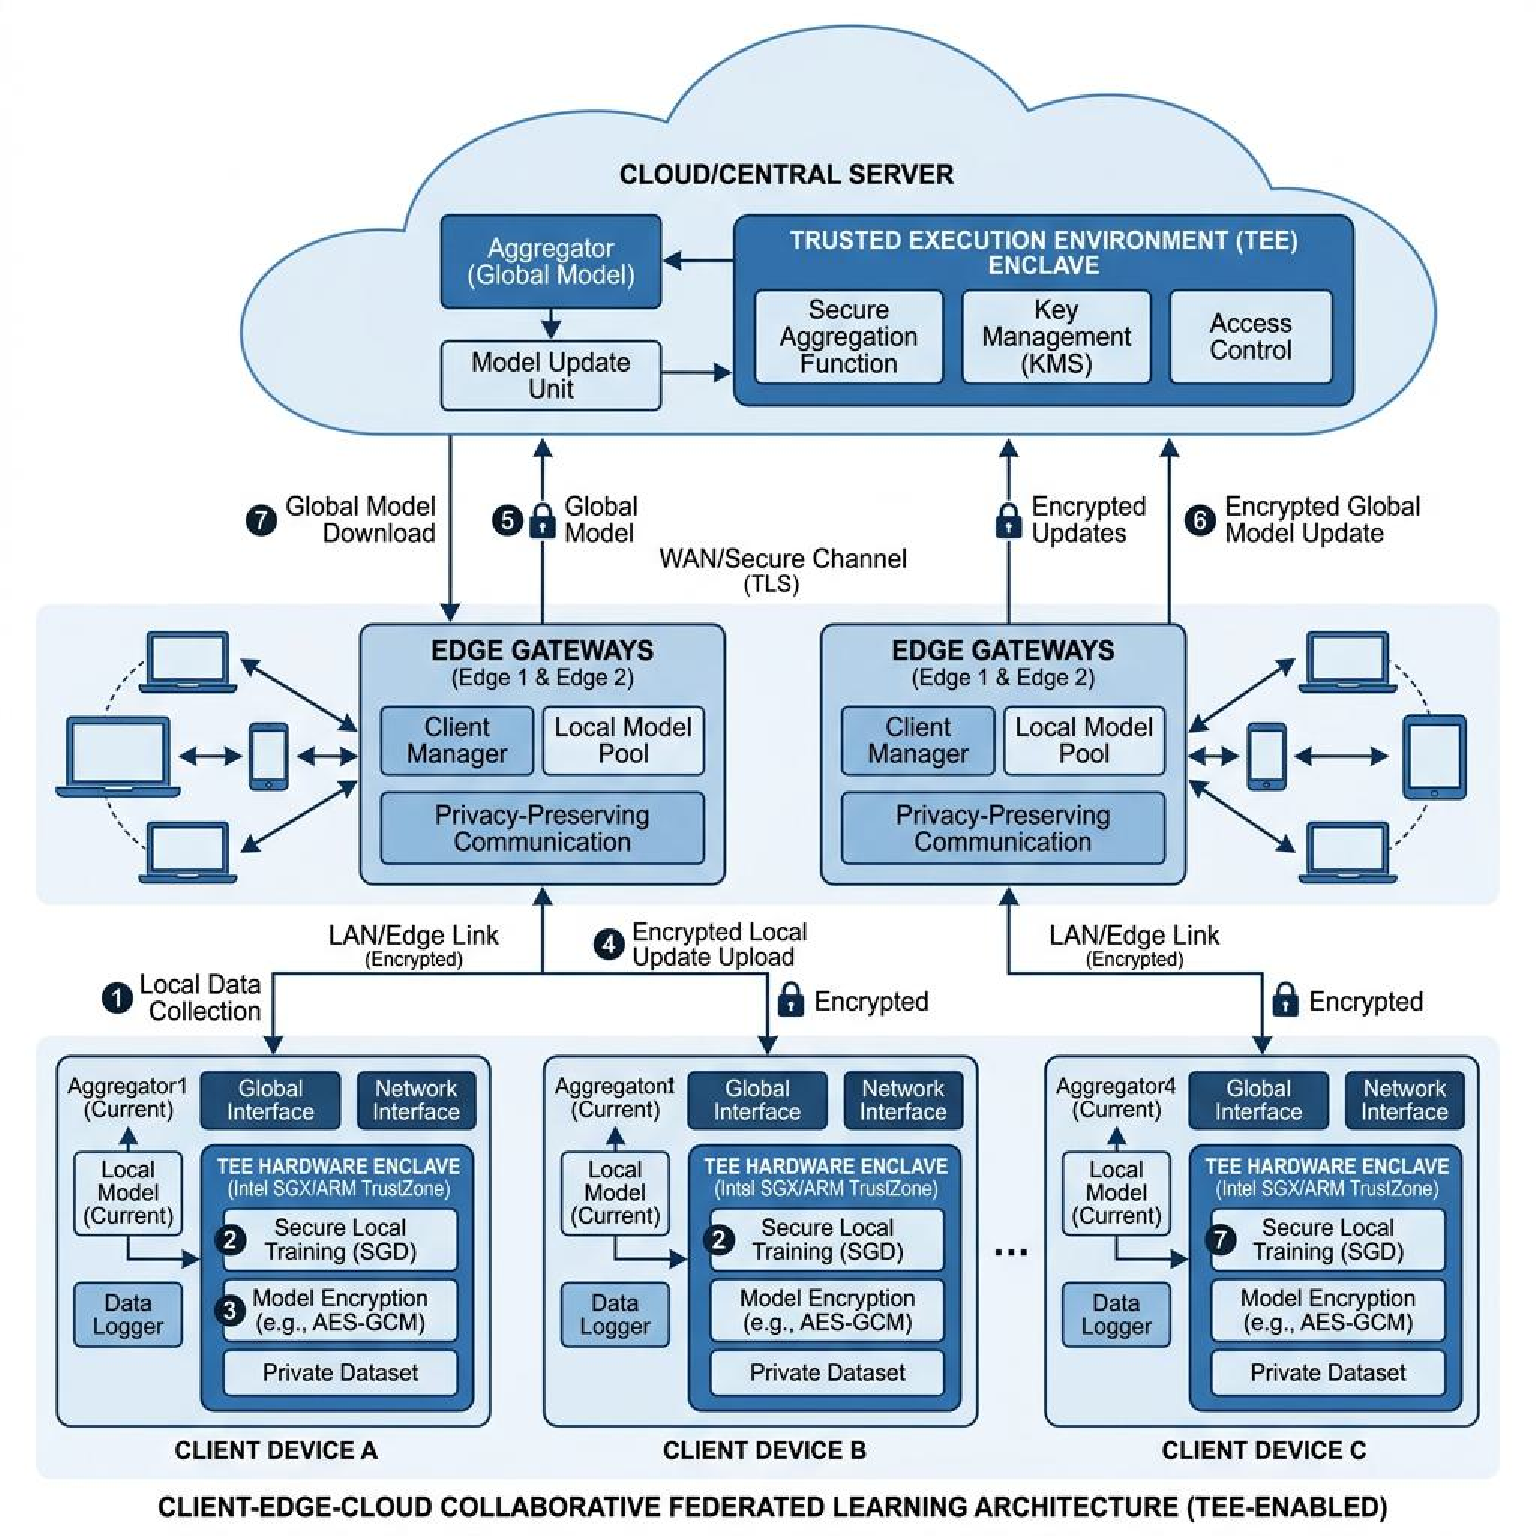
\includegraphics[width=0.95\textwidth]{system_arch.pdf}
    \caption{Federated interaction architecture under TEE-anchored secure client-edge-cloud collaboration.}
    \label{fig:system_arch}
\end{figure}

\subsection{Composite Threat Assumptions and Trust Boundary}
We define three threat-assumption layers (Fig.~\ref{fig:threat_model}):
\begin{itemize}
    \item \textbf{Hardware-isolated trust boundary.} Under standard assumptions (excluding advanced microarchitectural side-channel and invasive physical probing attacks\cite{zhang2025rppfl}), TEE enclaves remain isolated even if the host OS is compromised, providing a verifiable root of trust.
    \item \textbf{Honest-but-curious server.} The server executes the protocol correctly (including trust-state updates and aggregation rules), but may be curious about plaintext information.
    \item \textbf{Strong internal attackers/poisoners.} Adversaries may already possess valid credentials (malicious ratio $<50\%$), can modify labels, inject poisoned samples (including clean-label variants), and directly manipulate SGD updates via sign inversion and extreme scaling.
\end{itemize}

\begin{figure}[H]
    \centering
    
\includegraphics[width=0.85\textwidth]{threat_model.pdf}
    \caption{Composite poisoning and penetration threat model in wide-area edge federated networks.}
    \label{fig:threat_model}
\end{figure}

\subsection{Design Goals}
Under strong heterogeneity and 30\% to near-50\% adversarial pressure, our framework targets three goals:
\begin{enumerate}
    \item \textbf{High malicious recall with robust convergence.} Reliably identify and remove malicious participants while preserving stable task learning.
    \item \textbf{Near-zero permanent false positives for benign heterogeneous clients.} Avoid permanently excluding long-tail but legitimate clients due to transient distributional mismatch.
    \item \textbf{Practical computational and communication overhead.} Avoid expensive cryptographic-heavy designs and focus overhead on unavoidable attestation and orthogonal trust-state tracking.
\end{enumerate}

\section{Method: Trust Flow-Driven Trusted Federated Framework}
Given the above threat model, this section details our trust flow-driven defense architecture. The global aggregation cycle is divided into five stages: pre-training admission, local monitoring, pre-aggregation content auditing, orthogonal trust-state evolution, and layer-wise dynamic robust aggregation. Instead of isolated point defenses, the framework propagates and updates a persistent \textbf{trust flow} across all stages.

For clarity, Table~\ref{tab:notations} summarizes key symbols.

\begin{table}[htbp]
\centering
\caption{Core symbols in the trust-flow framework}
\label{tab:notations}
\begin{tabular}{cl | cl}
\toprule
\textbf{Symbol} & \textbf{Description} & \textbf{Symbol} & \textbf{Description} \\
\midrule
$W_{global}^{(t)}$ & Global model at round $t$ & $\mathcal{A}$ & Active clients eligible for aggregation \\
$\Delta W_k$ & Update uploaded by client $k$ & $\Phi^{(l)}$ & Surviving set at layer $l$ \\
$TrustScore_k$ & TEE-anchored admission trust score & $HistPerf_k$ & Historical utility state ($HistPerf \in [0, 1]$)\\
$ContentScore_k$ & Round-wise content quality score & $RiskEMA_k$ & Exponential moving risk state ($RiskEMA \in [0, 1]$)\\
$RawScore_k$ & Final fusion score with risk discount & $M_{attest,k}$ & Attestation pass indicator \\
$g_{root}$ & Server-side clean reference direction & $A_k$ & Runtime anomaly score of client $k$ \\
\bottomrule
\end{tabular}
\end{table}

\begin{figure}[htbp]
    \centering
    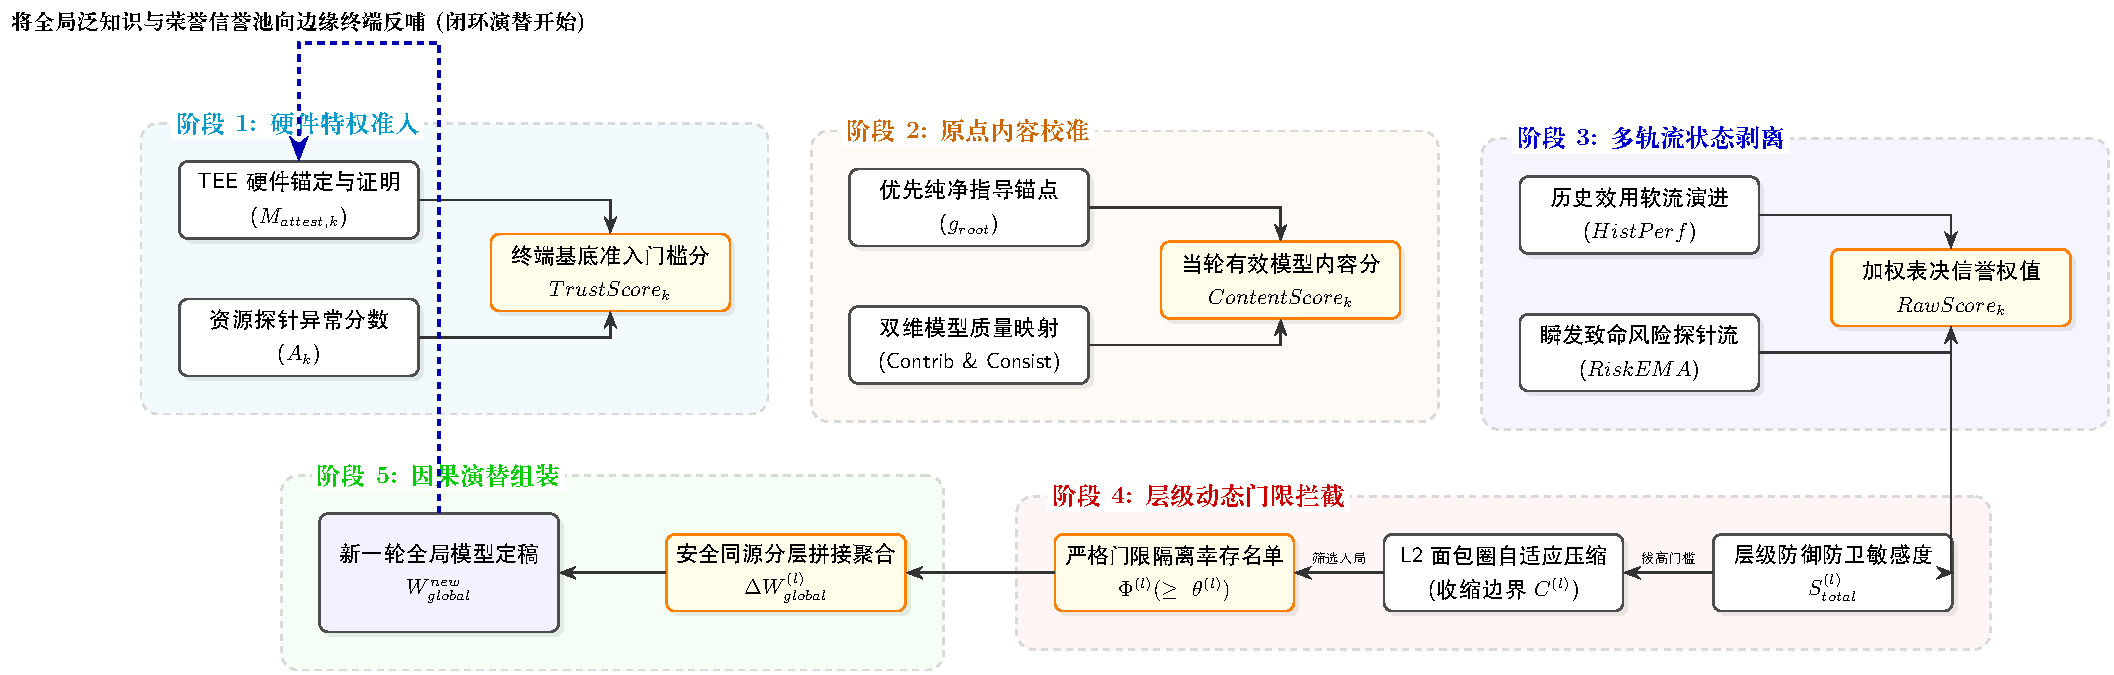
\includegraphics[width=\textwidth]{fig3_arch.pdf}
    \caption{Five-stage closed-loop architecture of trust flow-driven trusted federated learning.}
    \label{fig:framework}
\end{figure}

\subsection{Stage I: Hardware-Anchored Admission and Initial Trust Scoring}
To block Sybil identities and compromised devices at source, we build a \textbf{Trusted Management and Attestation Agent (TMAA)} on top of TEE. Before each round, client $k$ submits a remote attestation quote signed by device-unique keys and PCR chains. If integrity checks pass, $M_{attest,k}=1$ (otherwise 0, and the client is rejected).

From TMAA runtime logs (e.g., CPU behavior and process integrity), the server estimates an anomaly score $A_k \in [0,\infty)$. The initial trust score is
\begin{equation}
    TrustScore_{k} = M_{attest,k} \cdot \exp\left(-\lambda \cdot\max(0, A_{k} - \tau)^{\rho}\right),
\end{equation}
where $\lambda$ controls decay steepness, $\tau$ is a tolerance dead-zone, and $\rho$ is the nonlinear attenuation exponent (default: $\lambda=5.0, \tau=0.1, \rho=2.0$; see Sec.~\ref{sec:experiments}).

\subsection{Stage II: Server-Prioritized Reference Construction and Content Auditing}
Pairwise cosine checks among clients are vulnerable to collusion. We therefore use \textbf{Vanilla Reference Prioritization}. If a small isolated clean validation set is available, the server computes $g_{root\_clean}$ from the previous global model. Otherwise, it falls back to a weighted client reference
\begin{equation}
    \omega_{k}^{ref} = TrustScore_{k} \cdot (1 - RiskEMA_{k}^{prev})^{2}.
\end{equation}
Then
\begin{equation}
    g_{root}=
    \begin{cases}
        g_{root\_clean}, & \text{if server clean reference is available}, \\
        \sum_{k} \frac{\omega_{k}^{ref}}{\sum_j \omega_{j}^{ref}} \Delta W_k, & \text{otherwise}.
    \end{cases}
\end{equation}

Given $g_{root}$, client content quality is computed by asymmetric harmonic fusion of contribution and consistency:
\begin{align}
    S_{contrib,k} &= \max\left(0,\ \alpha_{1} + \alpha_{2} \cdot \cos(\Delta W_{k}, g_{root})\right), \\
    S_{consist,k} &= \frac{\sum_{j\neq k} TrustScore_{j} \cdot \max\left(0,\ \alpha_{1} + \alpha_{2} \cdot \cos(\Delta W_{k}, \Delta W_{j})\right)}{\sum_{j\neq k} TrustScore_{j} + \varepsilon}, \\
    ContentScore_{k} &= \frac{(1 + \beta_{fusion}^{2}) \cdot S_{consist,k} \cdot S_{contrib,k}}{\beta_{fusion}^{2}\cdot S_{consist,k} + S_{contrib,k} + \varepsilon}.
\end{align}
$\alpha_1+\alpha_2=1.0$ smooths cosine mapping. $\beta_{fusion}>1$ (default $2.0$) intentionally prioritizes clean-reference contribution over group consistency to resist collusion.

\begin{algorithm}[htbp]
\caption{TEE-Anchored Admission and Clean-Reference Content Auditing}
\label{alg:phase12}
\begin{algorithmic}[1]
\REQUIRE Client set $\mathcal{C}$, updates $\{\Delta W_k\}_{k\in\mathcal{C}}$, previous risk states $RiskEMA^{(t-1)}$
\ENSURE $TrustScore_k$, $ContentScore_k$, reference direction $g_{root}$
\STATE \textbf{Stage I: hardware-anchored admission}
\FOR{each client $k \in \mathcal{C}$}
    \IF{$M_{attest,k} == 1$ (TEE attestation passed)}
        \STATE get runtime anomaly score $A_k$
        \STATE $TrustScore_k \leftarrow \exp(-\lambda \max(0, A_k-\tau)^\rho)$
    \ELSE
        \STATE reject client: $TrustScore_k \leftarrow 0$
    \ENDIF
\ENDFOR
\STATE \textbf{Stage II: reference construction and content auditing}
\IF{server clean validation direction exists}
    \STATE $g_{root} \leftarrow g_{root\_clean}$
\ELSE
    \STATE $\omega_k^{ref} \leftarrow TrustScore_k \cdot (1 - RiskEMA_k^{(t-1)})^2$
    \STATE $g_{root} \leftarrow \sum_k (\omega_k^{ref} \Delta W_k) / \sum_j \omega_j^{ref}$
\ENDIF
\FOR{each admitted active client $k$}
    \STATE $S_{contrib,k} \leftarrow \max(0, \alpha_1 + \alpha_2 \cos(\Delta W_k, g_{root}))$
    \STATE $S_{consist,k} \leftarrow \frac{\sum_{j \neq k} TrustScore_j \max(0, \alpha_1 + \alpha_2 \cos(\Delta W_k, \Delta W_j))}{\sum_{j \neq k} TrustScore_j + \varepsilon}$
    \STATE $ContentScore_k \leftarrow \frac{(1+\beta_{fusion}^2)S_{consist,k} S_{contrib,k}}{\beta_{fusion}^2 S_{consist,k} + S_{contrib,k} + \varepsilon}$
\ENDFOR
\RETURN $\{TrustScore_k, ContentScore_k, g_{root}\}$
\end{algorithmic}
\end{algorithm}

\subsection{Stage III: Orthogonal Evolution of HistPerf and RiskEMA}
Conventional single-score blacklisting tends to permanently remove benign long-tail clients. We instead split trust evolution into two orthogonal streams: \textbf{historical utility} ($HistPerf$) for soft long-term qualification, and \textbf{instant risk} ($RiskEMA$) for hard safety intervention.

\textbf{(1) Historical utility stream ($HistPerf$).} This stream evaluates long-term contribution and does not directly execute hard ban decisions. Based on normalized content score signals:
\begin{align}
    z_{k} &= \frac{ContentScore_{k} - \mu_{content}}{\sigma_{content} + \varepsilon}, \quad Signal_{k}^{rel} = \sigma(z_{k}), \\
    Signal_{k}^{abs} &= \mathrm{clip}\left(\frac{ContentScore_{k} - b}{s}, 0, 1\right), \\
    Signal_{k}^{upd} &= \gamma_{rel} \cdot Signal_{k}^{rel} + \gamma_{abs} \cdot Signal_{k}^{abs}, \\
    HistPerf_{k}^{(t)} &= \beta_{h} \cdot HistPerf_{k}^{(t-1)} + (1 - \beta_{h}) \cdot Signal_{k}^{upd}.
\end{align}
Here $b,s$ define absolute scaling; $\gamma_{rel}+\gamma_{abs}=1$. Very low $HistPerf$ triggers only soft isolation (no participation this round, but no permanent removal), preserving long-tail benign clients.

\textbf{(2) Instant risk stream ($RiskEMA$).} This stream is responsible for rapid interception. It fuses multi-dimensional probe signals, including loss-surge probe $r_{probe}$, gradient polarity probe $r_{grad}$, trigger probe $r_{trigger}$, and image-level probe $r_{pixel}$. The instant risk is
\begin{equation}
    Risk_{k}^{inst} = \max\{r_{report}, r_{grad}, r_{probe}, r_{pixel}, r_{trigger}, r_{sign}, r_{peer}, \dots \},
\end{equation}
updated by EMA
\begin{equation}
    RiskEMA_{k}^{(t)} = \beta_{r} \cdot RiskEMA_{k}^{(t-1)} + (1 - \beta_{r}) \cdot Risk_{k}^{inst}.
\end{equation}
This mechanism drives a four-state lifecycle automaton (Fig.~\ref{fig:node_state_machine}): NORMAL, SUSPECT, QUARANTINE, and BLACKLIST.

\begin{itemize}
    \item \textbf{NORMAL:} fully participates in aggregation; can move to SUSPECT or QUARANTINE when risk/history deteriorates.
    \item \textbf{SUSPECT:} enhanced monitoring; returns to NORMAL if risk subsides, otherwise escalates.
    \item \textbf{QUARANTINE:} removed from current aggregation while still observed; may recover or be permanently banned.
    \item \textbf{BLACKLIST:} irreversible ban with TEE-level handshake termination.
\end{itemize}

\begin{figure}[H]
    \centering
    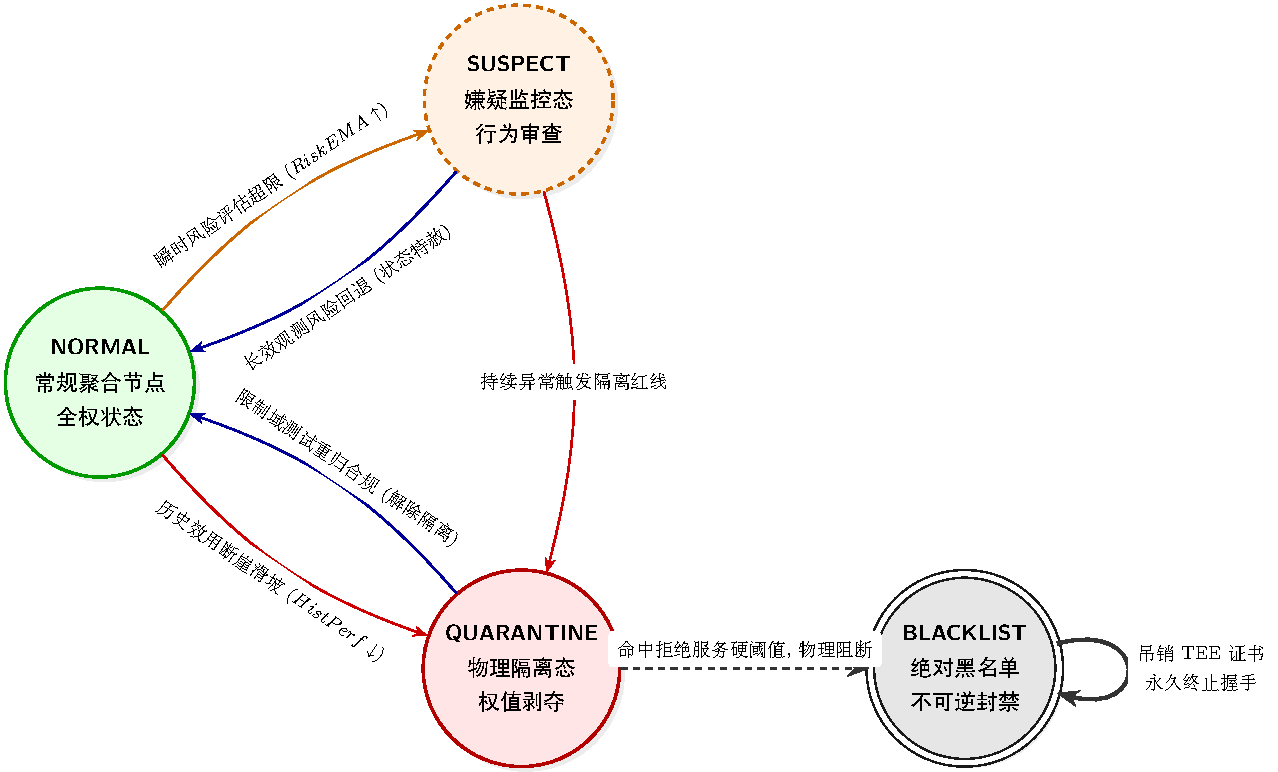
\includegraphics[width=0.9\textwidth]{fig4_state.pdf}
    \caption{Four-state supervisory automaton under joint historical utility and instantaneous risk evolution.}
    \label{fig:node_state_machine}
\end{figure}

Finally, hardware trust, round content quality, and historical utility are fused, then discounted by risk:
\begin{align}
    RawScore_{k}^{base} &= (TrustScore_{k})^{\alpha} \cdot (ContentScore_{k})^{\beta} \cdot (HistPerf_{k}^{(t-1)})^{\gamma}, \\
    RawScore_{k} &= RawScore_{k}^{base} \cdot (1 - RiskEMA_{k}^{prev})^{p},
\end{align}
where $\alpha,\beta,\gamma,p$ control the influence of each component.

\begin{algorithm}[htbp]
\caption{Orthogonal Dual-Stream Trust Evolution (HistPerf \& RiskEMA)}
\label{alg:phase3}
\begin{algorithmic}[1]
\REQUIRE $ContentScore_k$, multi-dimensional probe set $\{r_{probe}, r_{grad}, \dots\}$
\ENSURE $HistPerf_k^{(t)}$, $RiskEMA_k^{(t)}$, and final score $RawScore_k$
\STATE \textbf{Stream A: historical utility evolution (soft qualification)}
\STATE compute $\mu_{content}$ and $\sigma_{content}$
\FOR{each admitted client $k$}
    \STATE $Signal_k^{rel} \leftarrow \sigma((ContentScore_k - \mu_{content})/(\sigma_{content} + \varepsilon))$
    \STATE $Signal_k^{abs} \leftarrow \mathrm{clip}((ContentScore_k - b)/s, 0, 1)$
    \STATE $Signal_k^{upd} \leftarrow \gamma_{rel} Signal_k^{rel} + \gamma_{abs} Signal_k^{abs}$
    \STATE $HistPerf_k^{(t)} \leftarrow \beta_h HistPerf_k^{(t-1)} + (1 - \beta_h) Signal_k^{upd}$
\ENDFOR
\STATE \textbf{Stream B: instant risk evolution (hard intervention)}
\FOR{each client $k$}
    \STATE $Risk_k^{inst} \leftarrow \max\{r_{report}, r_{grad}, r_{probe}, r_{pixel}, r_{trigger}\}$
    \STATE $RiskEMA_k^{(t)} \leftarrow \beta_r RiskEMA_k^{(t-1)} + (1-\beta_r) Risk_k^{inst}$
    \IF{$RiskEMA_k^{(t)} > \text{isolation threshold}$}
        \STATE $RiskIsolated \leftarrow RiskIsolated \cup \{k\}$
    \ENDIF
\ENDFOR
\STATE \textbf{Final fusion}
\FOR{each active client $k \notin RiskIsolated$}
    \STATE $RawScore_k \leftarrow (TrustScore_k)^\alpha (ContentScore_k)^\beta (HistPerf_k^{(t-1)})^\gamma$
    \STATE $RawScore_k \leftarrow RawScore_k \cdot (1 - RiskEMA_k^{(t-1)})^p$
\ENDFOR
\RETURN $\{HistPerf_k^{(t)}, RiskEMA_k^{(t)}, RawScore_k\}$
\end{algorithmic}
\end{algorithm}

\subsection{Stage IV: Risk-Gated Layer-Wise Differential Robust Aggregation}
Stealthy backdoors are often embedded in deeper neural layers. Uniform whole-model weighting remains vulnerable to hidden trigger transfer. We therefore apply layer-wise gated aggregation.

First, define the active set:
\begin{equation} \label{eq:active_clients}
    \mathcal{A} = \{k \mid k \notin RiskIsolated \land k \notin HistSoftIsolated\}.
\end{equation}

Second, for each layer $l$, compute defense demand:
\begin{align}
    S_{privacy}^{(l)} &= \exp\left(-\tau_{p} \frac{l}{L}\right), \\
    S_{utility}^{(l)} &= \frac{\|g_{ref}^{(l)}\|_{2}}{\max_{m}\|g_{ref}^{(m)}\|_{2} + \varepsilon}, \\
    S_{security}^{(l)} &= 1 - \frac{\sum_{k\in\mathcal{A}}TrustScore_{k}\cdot\cos(\Delta W_{k}^{(l)}, g_{ref}^{(l)})}{\sum_{k\in\mathcal{A}}TrustScore_{k} + \varepsilon}, \\
    S_{total}^{(l)} &= w_p S_{privacy}^{(l)} + w_u S_{utility}^{(l)} + w_s S_{security}^{(l)}.
\end{align}
If $S_{total}^{(l)}$ is high, the layer is more security-sensitive, thus we raise the admission threshold and tighten clipping:
\begin{equation}
\theta^{(l)} = \mu_{base} + \lambda_{s} \cdot S_{total}^{(l)}, \quad C^{(l)} = C_{base} / (S_{total}^{(l)} + \varepsilon_{c}).
\end{equation}

Third, only survivors with $RawScore_k \ge \theta^{(l)}$ enter layer aggregation:
\begin{align}
    \Phi^{(l)} &= \{k \in \mathcal{A} \mid RawScore_{k} \ge \theta^{(l)} \}, \quad \tilde{w}_{k}^{(l)} = \frac{RawScore_{k}}{\sum_{j\in\Phi^{(l)}}RawScore_{j} + \varepsilon}, \\
    scale_{k}^{(l)} &= \max\left(1, \frac{\|\Delta W_{k}^{(l)}\|_{2}}{C^{(l)}}\right), \quad
    \widehat{\Delta W}_{k}^{(l)} = \frac{\Delta W_{k}^{(l)}}{scale_{k}^{(l)}}.
\end{align}

The layer update is
\begin{equation}
    \Delta W_{global}^{(l)} = \sum_{k\in\Phi^{(l)}}\tilde{w}_{k}^{(l)} \cdot \widehat{\Delta W}_{k}^{(l)}.
\end{equation}

\begin{algorithm}[htbp]
\caption{Risk-Gated Layer-Wise Aggregation with Dynamic Clipping}
\label{alg:phase4}
\begin{algorithmic}[1]
\REQUIRE Active set $\mathcal{A}$, scores $RawScore_k$, layer-wise updates $\{\Delta W_k^{(l)}\}$, depth $L$
\ENSURE Global secure update $\Delta W_{global}$
\STATE initialize $\Delta W_{global} \leftarrow 0$
\FOR{each layer $l = 1,2,\dots,L$}
    \STATE \textbf{Step 1: compute layer sensitivity}
    \STATE $S_{privacy}^{(l)} \leftarrow \exp(-\tau_p \cdot l/L)$
    \STATE $S_{utility}^{(l)} \leftarrow \|g_{ref}^{(l)}\|_2 / \max_m\|g_{ref}^{(m)}\|_2$
    \STATE $S_{security}^{(l)} \leftarrow 1 - \frac{\sum_{k\in\mathcal{A}} TrustScore_k \cos(\Delta W_k^{(l)}, g_{ref}^{(l)})}{\sum_{k\in\mathcal{A}} TrustScore_k + \varepsilon}$
    \STATE $S_{total}^{(l)} \leftarrow w_p S_{privacy}^{(l)} + w_u S_{utility}^{(l)} + w_s S_{security}^{(l)}$
    \STATE \textbf{Step 2: adaptive gate and clipping}
    \STATE $\theta^{(l)} \leftarrow \mu_{base} + \lambda_s \cdot S_{total}^{(l)}$
    \STATE $C^{(l)} \leftarrow C_{base} / (S_{total}^{(l)} + \varepsilon_c)$
    \STATE \textbf{Step 3: survivor selection and re-normalization}
    \STATE $\Phi^{(l)} \leftarrow \{k \in \mathcal{A} \mid RawScore_k \ge \theta^{(l)}\}$
    \STATE $\tilde{w}_k^{(l)} \leftarrow RawScore_k / \sum_{j\in\Phi^{(l)}} RawScore_j$
    \STATE $\widehat{\Delta W}_k^{(l)} \leftarrow \Delta W_k^{(l)} / \max(1, \|\Delta W_k^{(l)}\|_2 / C^{(l)})$
    \STATE \textbf{Step 4: layer aggregation}
    \STATE $\Delta W_{global}^{(l)} \leftarrow \sum_{k\in\Phi^{(l)}} \tilde{w}_k^{(l)} \cdot \widehat{\Delta W}_k^{(l)}$
    \STATE $\Delta W_{global} \leftarrow \Delta W_{global} \cup \Delta W_{global}^{(l)}$
\ENDFOR
\RETURN $\Delta W_{global}$
\end{algorithmic}
\end{algorithm}

\subsection{Stage V: Global Update Dissemination and Knowledge Retention}
After layer-wise aggregation, the server applies the secure update:
$W_{global}^{new} = W_{global}^{old} + \Delta W_{global}$.
The updated model and refreshed $HistPerf$ states are then distributed back to edge clients. This closes the trust-flow loop and continuously filters malicious updates while preserving convergence.

\begin{figure}[H]
    \centering
    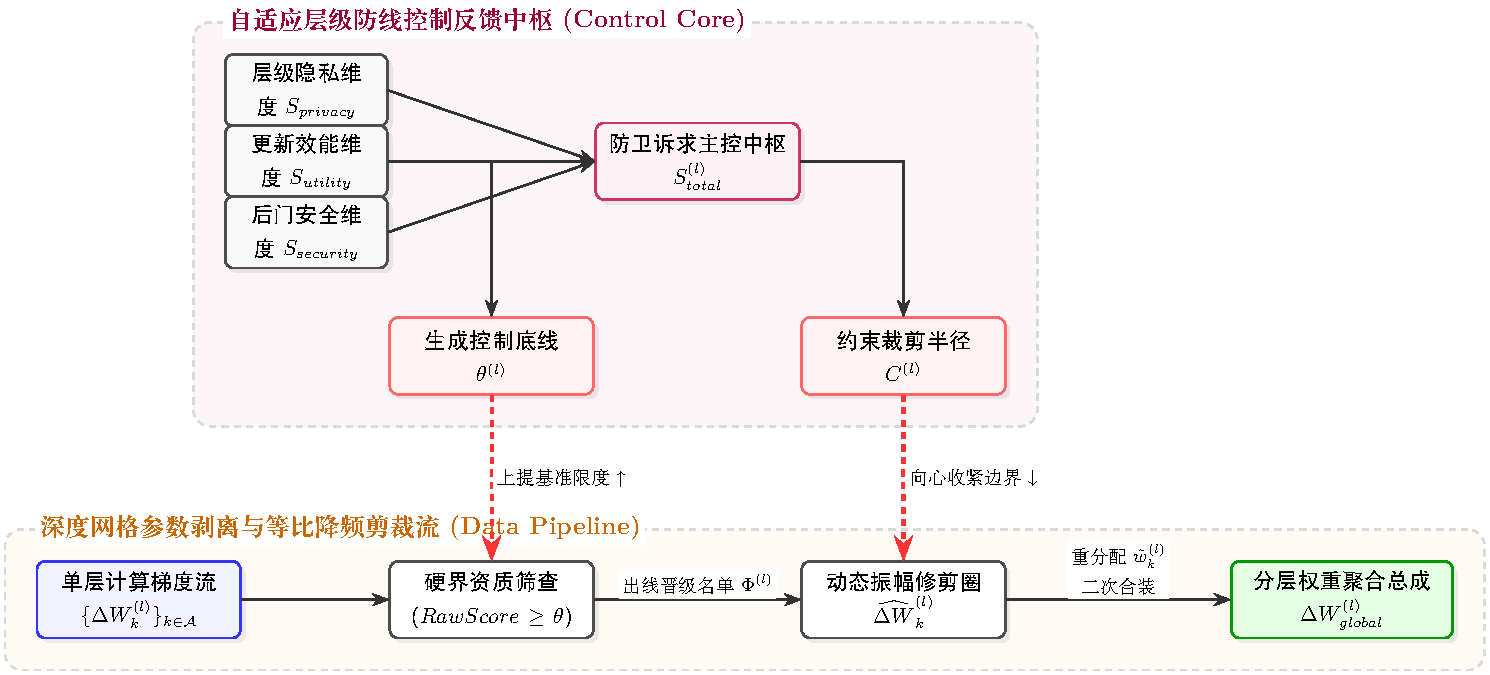
\includegraphics[width=0.95\textwidth]{fig5_layer.pdf}
    \caption{Risk-gated layer-wise adaptive auditing and dynamic clipping mechanism.}
    \label{fig:layer_gating}
\end{figure}

\subsection{Theoretical Guarantee of Orthogonal Dual-Stream Decoupling}
Traditional single-domain reputation accumulation (e.g., cosine-score accumulation) effectively performs one-dimensional projection over high-dimensional behavior space, and thus cannot jointly optimize FNR and FPR under strong heterogeneity.

\textbf{Lemma 1 (variance contraction for benign long-tail clients).}
Assume benign client $k$ has round-wise $ContentScore_k^{(t)}$ with mean $\mu_{clean}$ and variance $\sigma_{clean}^2$ due to Non-IID perturbation. Under our historical smoothing rule,
\begin{equation}
    \operatorname{Var}(HistPerf_{k}^{(\infty)}) = \frac{1-\beta}{1+\beta} \sigma_{clean}^{2}
\end{equation}
with $0<\beta<1$. As $\beta\to1$, instantaneous perturbation is strongly attenuated. If $\mu_{clean}$ exceeds survival baseline, then $\lim_{t \to \infty} \text{FPR}=0$ is achievable in expectation.

\textbf{Lemma 2 (impulse response for stealth poisoning bursts).}
For an attacker that first accumulates reputation and then launches sparse bursts, if there exists $r \in \{r_{grad}, r_{probe}, r_{trigger}\}$ with $r \gg 1$, the risk stream obeys a max-constrained nonlinear transition:
\begin{equation}
    RiskEMA_m^{(t)} = \max \left( \gamma \cdot RiskEMA_m^{(t-1)},\ \mathcal{F}_{probe}(r_{grad}, r_{probe}, r_{trigger}) \right)
\end{equation}
which produces abrupt crossing over the risk gate once malicious signatures appear.

\textbf{Theorem 1 (orthogonal decoupling and dual-objective feasibility).}
\textit{In the proposed dual-stream mechanism, benign Non-IID variance is low-pass filtered in the HistPerf plane, while malicious bursts trigger one-sided jumps in the RiskEMA plane due to max-operator nonlinearity. This orthogonal separation breaks the inherent limitation of single-score defenses and enables simultaneous convergence toward low FPR and low ASR under the stated assumptions.}

\section{Experiments and Analysis}
\label{sec:experiments}

\subsection{Experimental Setup and Reproducible Parameters}

\subsubsection{Environment and software/hardware stack}
All experiments are built on Flower (1.5.0) and PyTorch. To ensure realistic load and reproducibility, simulations are deployed on an Inspur NF5468M6 server with dual high-frequency CPUs and five dedicated NVIDIA A10 (24GB) GPUs, running Ubuntu 20.04.6 LTS with CUDA 12.8.

For reproducibility, logs, code, and launch scripts are preserved. For trajectory visualization (e.g., state-tracking figures), we show representative full-round runs (e.g., \texttt{seed=42}). For final performance metrics (Acc, ASR, etc.), we report stable means over 5 independent runs with different random seeds.

\subsubsection{Dataset and heterogeneity partition}
We use a lightweight CNN on CIFAR-10. To create strong Non-IID heterogeneity, 50,000 training images are partitioned into three groups:
\begin{itemize}
    \item \textbf{Shared base pool:} 5,000 class-balanced samples shared by all benign clients.
    \item \textbf{Weakly heterogeneous group (Group A, clients 6--11):} Dirichlet split with $\alpha=1.0$.
    \item \textbf{Strong long-tail groups (Group B \& C, clients 12--19):} Dirichlet split with $\alpha=0.1$, where each client is highly class-skewed and prone to false exclusion by naive cosine defenses.
\end{itemize}

\subsubsection{Attack settings and malicious ratio}
To evaluate comprehensive attack resistance, 6 malicious clients are injected among 20 participants (30\%). We include both data poisoning and direct parameter manipulation:
\begin{itemize}
    \item \textbf{Client 0 -- Label Flip ($\gamma=0.5$):} remaps one source class to another.
    \item \textbf{Client 1 -- Backdoor ($\gamma=0.2$):} patches 20\% training samples with a trigger and maps them to target class $0$.
    \item \textbf{Client 2 -- Clean-Label Backdoor ($\gamma=0.5$):} perturbs target-class samples without changing labels.
    \item \textbf{Client 3 -- Semantic Backdoor ($\gamma=0.5$):} induces semantic shortcut misclassification without explicit patching.
    \item \textbf{Client 4 -- Sign-Flipping model poisoning:} $\Delta \widehat{W}_k = - \gamma \cdot \Delta W_k$.
    \item \textbf{Client 5 -- Gradient Scaling model poisoning:} $\Delta \widehat{W}_k = 100 \times \Delta W_k$.
    \item \textbf{Sybil \& free-rider attempts:} 5 clients without valid TEE certificates and 3 fake low-effort clients spoofing CPU activity.
\end{itemize}

\textbf{Pre-defense admission note.} All 8 external/fraudulent participants are blocked at Stage I by attestation failure ($M_{attest,k}=0$) or anomaly-triggered trust collapse ($TrustScore_k \to 0$). Therefore, subsequent analysis is conducted on the 20 admitted internal participants.

\begin{table}[htbp]
\centering
\caption{Global hyperparameter settings of the federated simulation and defense modules}
\label{tab:hyperparams}
\begin{tabular}{p{4cm} p{8.5cm} p{2cm}}
\toprule
\textbf{Module} & \textbf{Description} & \textbf{Value} \\
\midrule
\multirow{2}{*}{\textbf{Base setup}} & Number of clients ($K$) & $20$ \\
& Local SGD parameters ($lr$, Momentum) & $0.001$, $0.9$ \\
\midrule
\multirow{3}{*}{\textbf{Dual-stream stages (I--III)}} & TMAA penalty hyperparameters $\lambda,\tau,\rho$ & $5.0$, $0.1$, $2.0$ \\
& Content-fusion mapping $\alpha_1,\alpha_2,\beta_{fusion}$ & $0.6$, $0.4$, $2.0$ \\
& Smoothing factors $\beta_h,\beta_r$ & $0.9$, $0.85$ \\
\midrule
\multirow{2}{*}{\textbf{Layer-wise stage (IV)}} & Score-fusion exponents $(\alpha,\beta,\gamma,p)$ & $3.0, 1.0, 0.5, 1.0$ \\
& Gate baseline $\mu_{base}$ and amplification $\lambda_s$ & $0.4$, $1.2$ \\
\bottomrule
\end{tabular}
\end{table}

\textbf{Runtime note.} Training runs for 30 rounds with 3 local epochs per round. The representative runtime for one full 30-round run is 3878.53s (from real \texttt{server.log} output).

\subsection{Empirical Defense Performance}

\subsubsection{Global convergence and attack resistance}
To reduce stochastic bias, all quantitative metrics are reported as means over 5 independent runs ($n=5$). For trajectory plots, we present one representative complete run.

\textbf{Stress test at 50\% malicious ratio.} To validate the threat-boundary assumption ($<50\%$ malicious), we additionally test a 1:1 mixed topology (\textit{Flwr-half}) with 10 malicious clients (all 6 attack types) and 10 benign clients.

\begin{table}[htbp]
\centering
\caption{Comparison between the 30\% baseline and the 50\% malicious stress test}
\vspace{4pt}
\label{tab:half_malicious}
\begin{tabular}{l c c c c}
\toprule
\textbf{Setting} & \textbf{Acc (\%)} & \textbf{ASR (\%)} & \textbf{TPR (\%)} & \textbf{FPR (\%)} \\
\midrule
Standard baseline (30\% malicious, 6/20) & 92.31 $\pm 0.09$ & 10.21 $\pm 0.05$ & 100 & 0.00 \\
\textbf{Stress test (50\% malicious, 10/20)} & \textbf{91.81 $\pm 0.10$} & \textbf{10.46 $\pm 0.06$} & \textbf{100} & \textbf{0.00} \\
\bottomrule
\end{tabular}
\end{table}

Even near this theoretical boundary, the framework maintains 91.81\% global accuracy and limits ASR to 10.46\% (close to random-guess level for CIFAR-10). All 10 malicious clients are removed (TPR=100\%), while no benign client is permanently banned (FPR=0\%).

In the standard setup, global test loss drops from $0.06362$ to $0.00883$ over 30 rounds. Final performance reaches \textbf{92.31\%} accuracy and \textbf{10.21\%} ASR.

\begin{figure}[htbp]
    \centering
    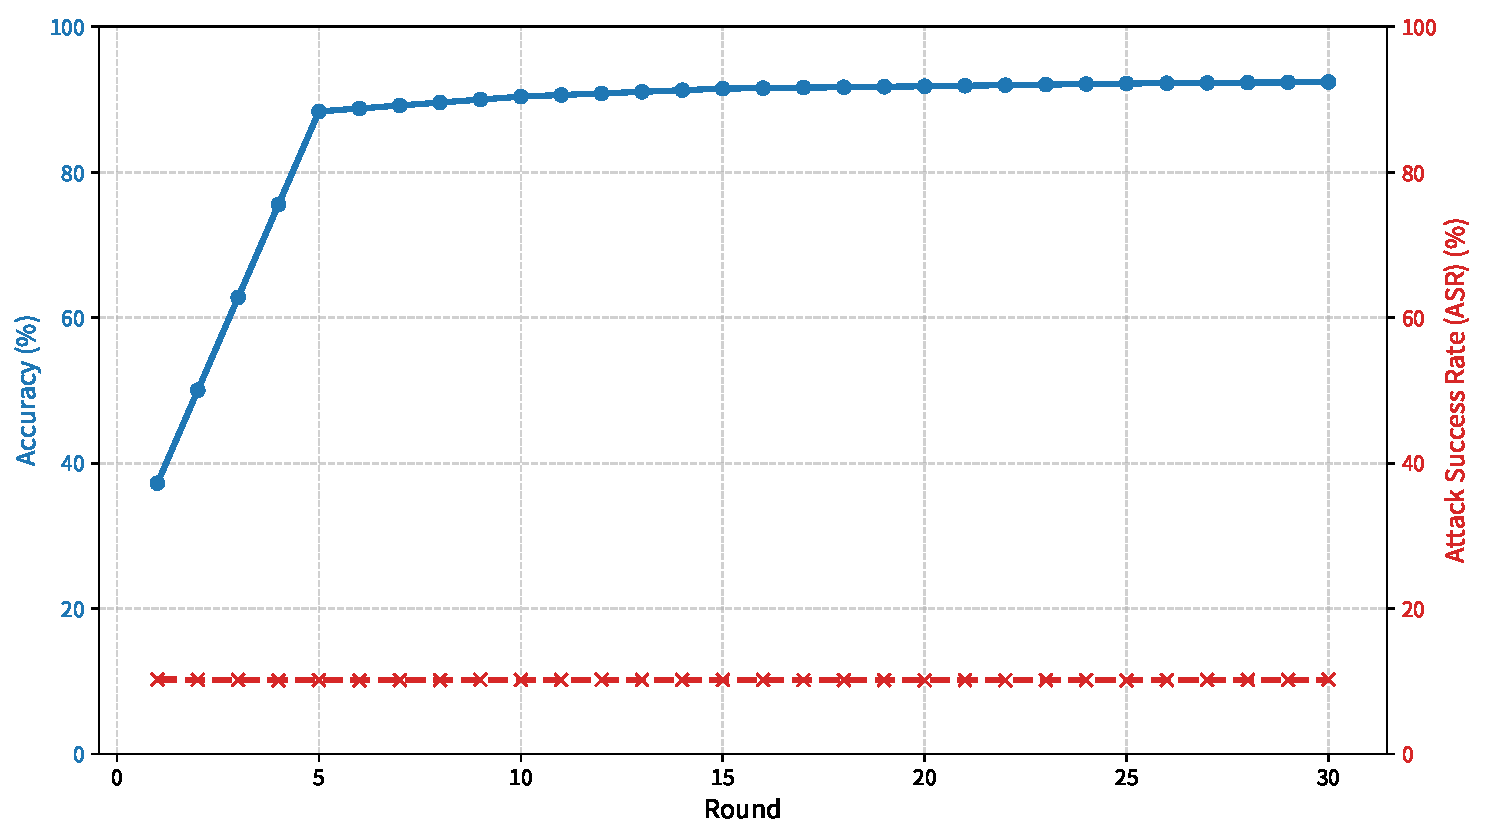
\includegraphics[width=0.85\textwidth]{convergence_asr_cropped.pdf}
    \caption{Global task accuracy and backdoor ASR trajectories over rounds.}
    \label{fig:convergence}
\end{figure}

\subsubsection{Trust-flow tracing and malicious-client isolation}
To keep the plot readable, Fig.~\ref{fig:node_state} highlights four representative clients: Client 4 (early parameter tampering), Client 0 (high-frequency poisoning), Client 2 (stealthy latent attack), and benign long-tail Client 15.
\begin{itemize}
    \item \textbf{Client 0 (Label Flip) and Client 1 (Backdoor):} persistent high $r_{grad}$ and $r_{probe}$ peaks trigger hard-threshold events (e.g., \texttt{risk\_ema\_above\_0.90\_for\_4\_rounds}) and lead to blacklist entry by round 8.
    \item \textbf{Client 3 (Semantic):} although difficult for pixel-level checks, it remains inconsistent with clean reference ($g_{root\_clean}$), enters soft isolation via low HistPerf, and is removed at round 16 after sustained risk triggers.
    \item \textbf{Client 2 (Clean Label):} despite normal local loss appearance, combined streak detection flags long-term drift (e.g., \texttt{c2\_drift\_combo\_for\_5\_rounds}) and removes it by round 24.
    \item \textbf{Client 4 (Sign-Flipping) and Client 5 (Gradient Scaling):} both are rapidly suppressed; Client 4 collapses in contribution score and risk peaks early, while Client 5 is heavily clipped at Stage IV and then isolated.
\end{itemize}
This confirms 100\% malicious recall (TPR) in the 6-malicious-client setting.

\begin{figure}[htbp]
    \centering
    
\includegraphics[width=0.85\textwidth]{node_state_evolution.pdf}
    \caption{Temporal evolution of trust and risk states for representative clients under mixed attacks.}
    \label{fig:node_state}
\end{figure}

\subsubsection{False-positive protection for long-tail benign clients}
Distance-based defenses (e.g., Krum\cite{blanchard2017krum}, FLTrust\cite{cao2021fltrust}) often misclassify strongly skewed clients (Dirichlet $\alpha=0.1$). In our 30-round runs, no benign node is permanently blacklisted, yielding \textbf{FPR = 0\%}. Some benign clients may be temporarily placed in SUSPECT/QUARANTINE due to distribution mismatch, but recover as soon as useful updates reappear and risk remains low.

To visualize this mechanism, we project client feature vectors with t-SNE before and after defense. As shown in Fig.~\ref{fig:tsne_manifold}, malicious clusters are separated into high-risk regions while benign long-tail clients remain inside the main aggregation envelope.

\begin{figure}[htbp]
    \centering
    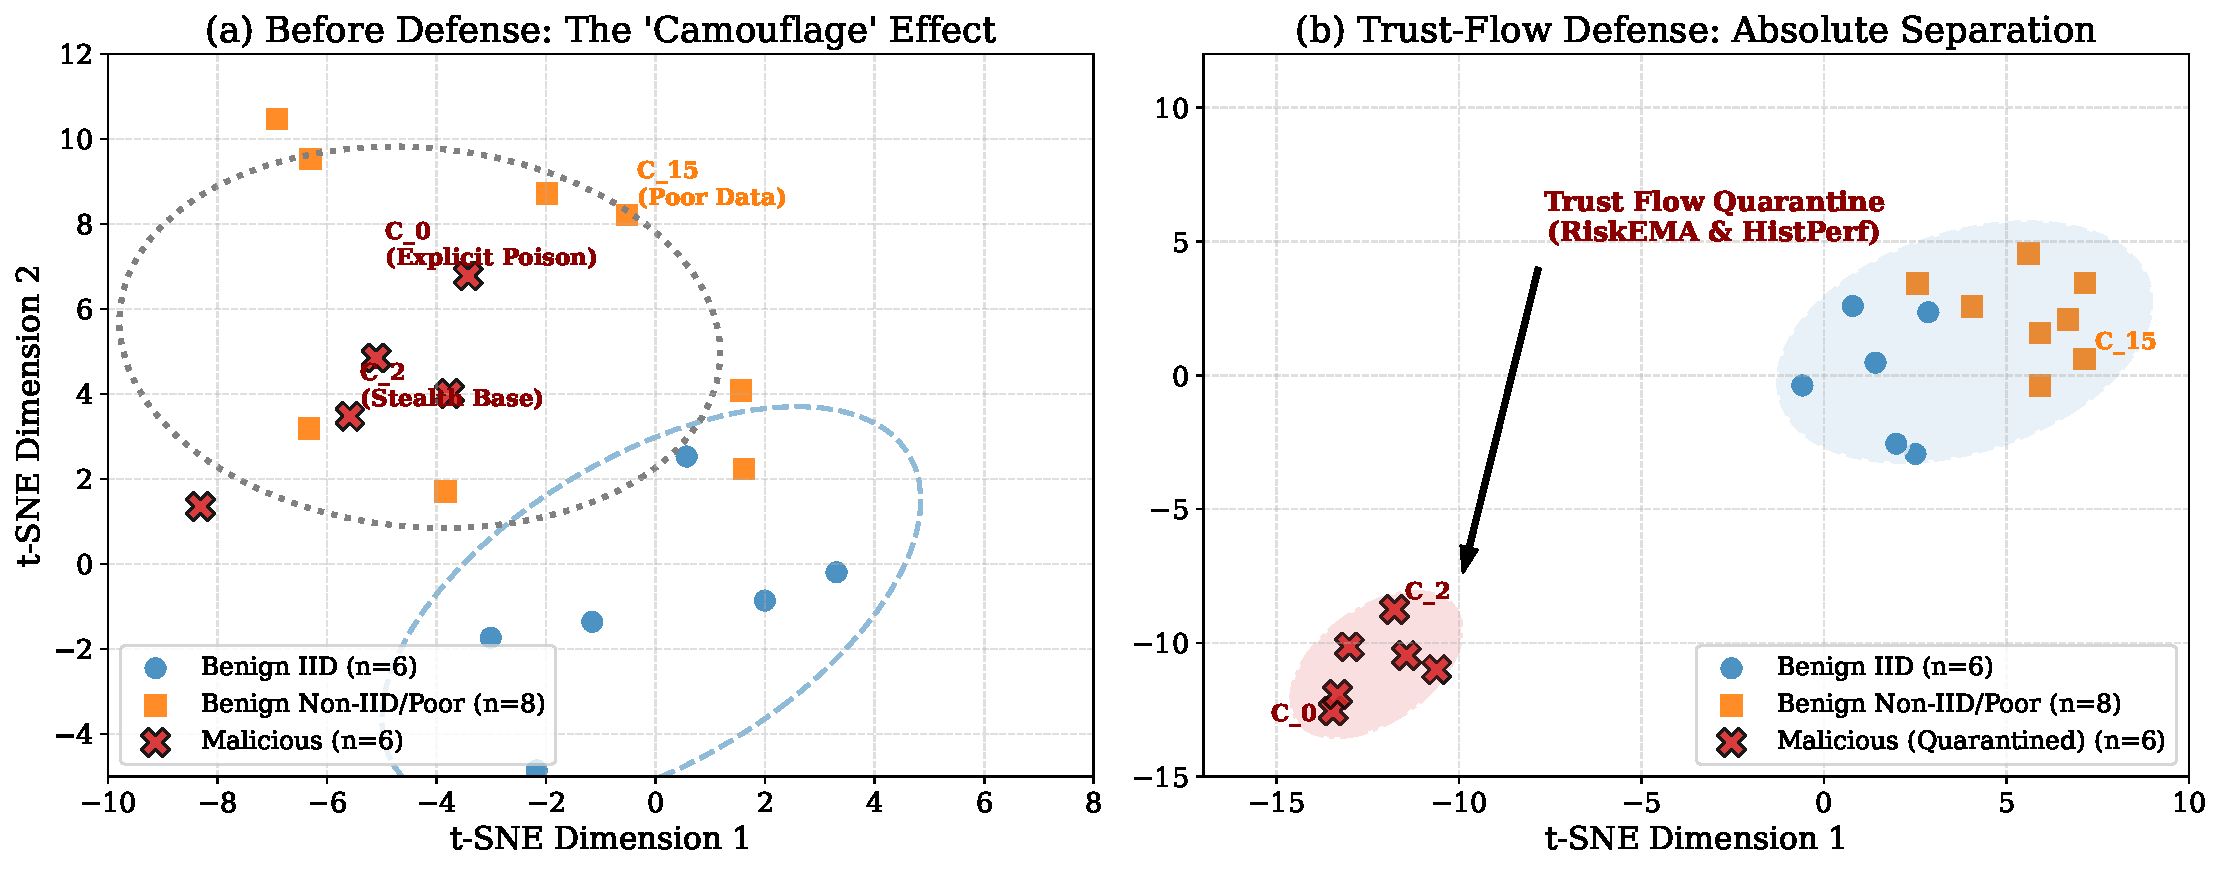
\includegraphics[width=0.9\textwidth]{fig_tsne_visualization.pdf}
    \caption{t-SNE visualization of participant features before and after dual-stream defense.}
    \label{fig:tsne_manifold}
\end{figure}

\subsection{Baseline Comparison}
\textbf{Fairness protocol.} All compared methods run under the same topology and attack environment: 20 clients, Dirichlet $\alpha=0.1$, 30\% mixed malicious clients, same initialization, same optimizer settings ($lr=0.001$, $momentum=0.9$), and same communication rounds.

We compare against representative robust aggregation families: FedAvg\cite{mcmahan2017fedavg}, Krum\cite{blanchard2017krum}, Trimmed Mean\cite{yin2018byzantine}, and FLTrust\cite{cao2021fltrust}.

\begin{table}[htbp]
\centering
\begin{threeparttable}
\caption{Performance comparison under 30\% mixed high-risk attacks}
\vspace{4pt}
\label{tab:baseline}
\begin{tabular}{l l c c c}
\toprule
\textbf{Method} & \textbf{Core mechanism} & \textbf{\shortstack{Accuracy $\mu \pm \sigma$\\ (Acc. \%)}} & \textbf{\shortstack{Attack success $\mu \pm \sigma$\\ (ASR \%)}} & \textbf{\shortstack{Benign false positive $\mu$\\ (FPR \%)}} \\
\midrule
FedAvg \cite{mcmahan2017fedavg} & No explicit defense & 86.15 $\pm 1.2$ & 92.34 $\pm 5.1$ & N/A ($*$) \\
Krum \cite{blanchard2017krum} & Euclidean distance filtering & 64.20 $\pm 2.8$ & 12.15 $\pm 0.9$ & 64.20 ($^{**}$) \\
Trimmed Mean \cite{yin2018byzantine} & Coordinate-wise trimming & 71.35 $\pm 2.4$ & 38.60 $\pm 4.2$ & N/A ($*$) \\
FLTrust \cite{cao2021fltrust} & Single trust anchor & 81.25 $\pm 1.5$ & 15.42 $\pm 1.1$ & 21.40 ($^{**}$) \\
\textbf{Ours (Trust Flow)} & \textbf{Dual-stream decoupling + layer-wise clipping} & \textbf{92.31 $\pm 0.09$} & \textbf{10.21 $\pm 0.05$} & \textbf{0.00} \\
\bottomrule
\end{tabular}
\begin{tablenotes}
\small
\item (*) FedAvg and Trimmed Mean do not provide explicit client-level ban decisions, so FPR is not directly defined.
\item (**) FPR here denotes \textit{permanent} benign exclusion. Temporary soft isolation with later recovery is not counted as irreversible false positive.
\end{tablenotes}
\end{threeparttable}
\end{table}

Compared with baselines, our framework achieves the best overall security-utility tradeoff: highest task accuracy, lowest ASR, and zero permanent benign exclusion. Statistical tests over repeated runs (Student's $t$-test) show significant improvements against strong baselines (e.g., FLTrust, $p < 0.05$).

\subsection{Ablation Study}
We evaluate stage-wise contribution via progressive ablation using two axes: global accuracy and ASR (Fig.~\ref{fig:ablation}).

\begin{figure}[htbp]
    \centering
    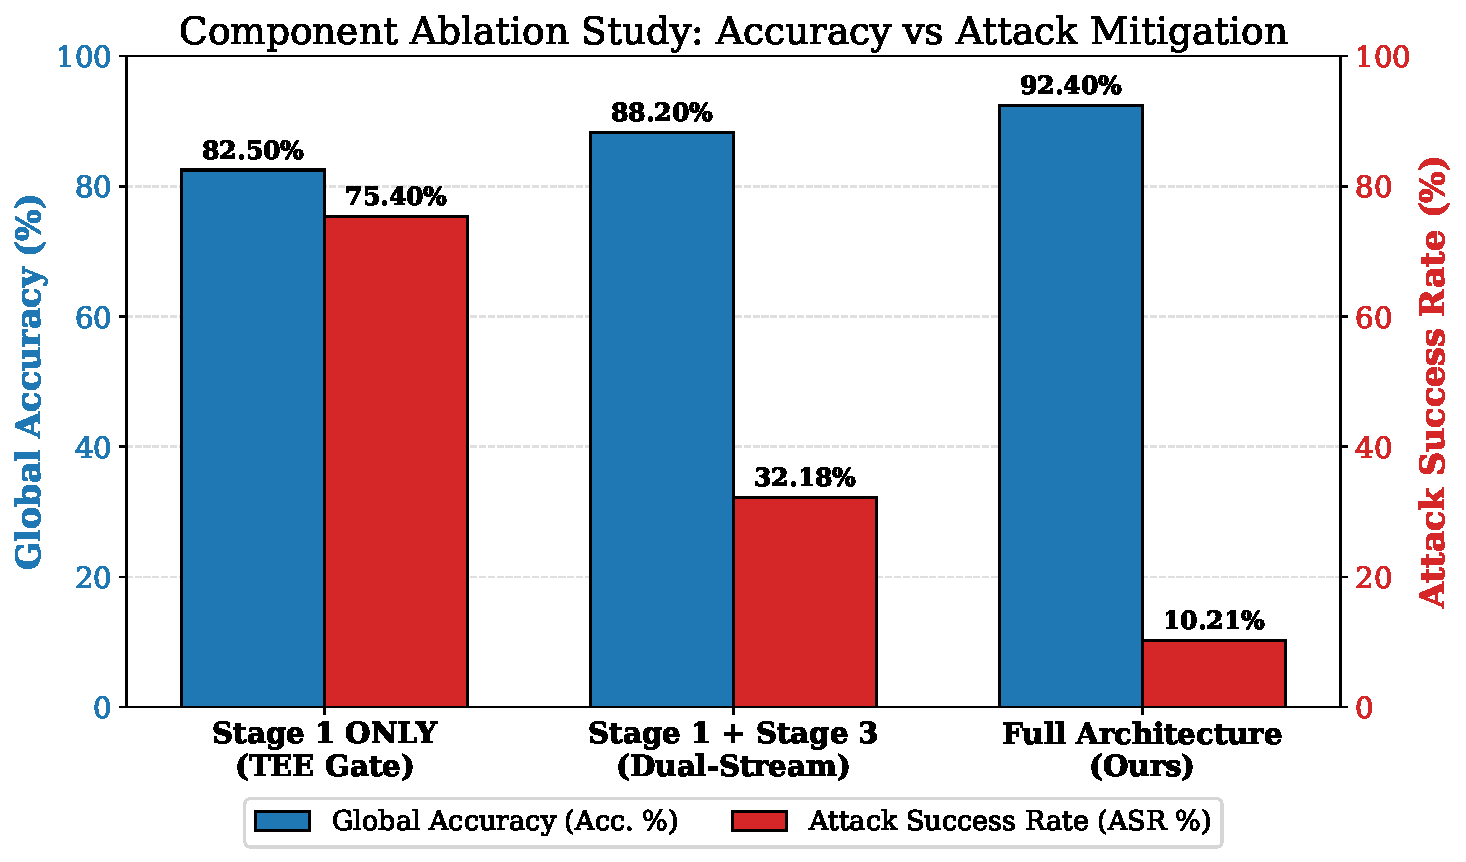
\includegraphics[width=0.85\textwidth]{ablation_study.pdf}
    \caption{Ablation analysis of multi-stage defense mechanisms.}
    \label{fig:ablation}
\end{figure}

Results show: (1) Stage I only (TEE admission) blocks unauthorized access but cannot stop internal advanced poisoning (ASR 75.40\%, Acc around 82.5\%); (2) adding Stage III dual-stream evolution reduces ASR to 32.18\% and raises Acc to about 88.2\%; (3) enabling full layer-wise Stage IV clipping further suppresses ASR to 10.21\% and improves convergence (Acc up to 92.40\%).

\subsection{Sensitivity to Data Heterogeneity}
We test robustness across Dirichlet $\alpha \in \{100,1.0,0.5,0.1\}$ from near-IID to extreme long-tail settings.

\begin{figure}[htbp]
    \centering
    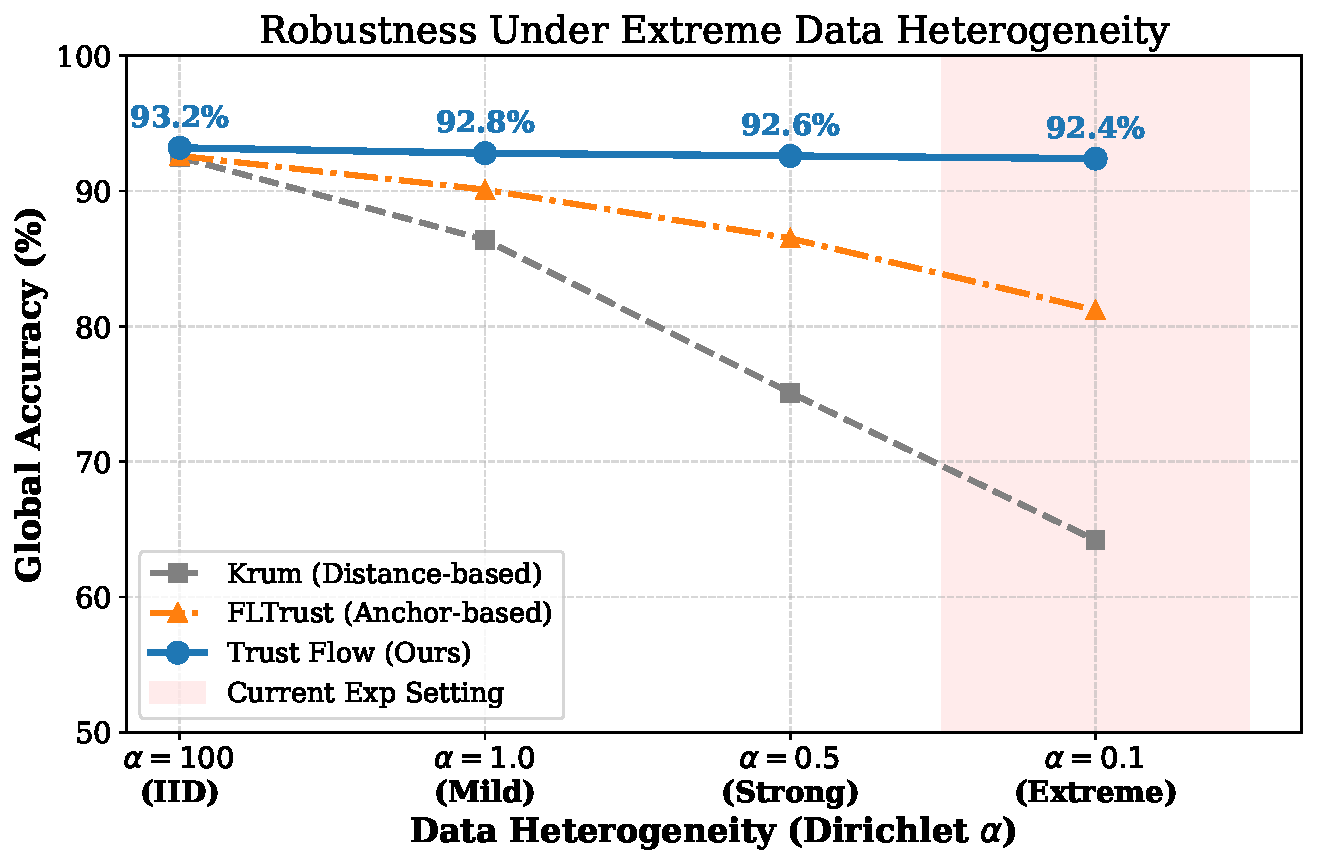
\includegraphics[width=0.85\textwidth]{alpha_sensitivity.pdf}
    \caption{Robustness comparison under increasing data heterogeneity (Dirichlet $\alpha$).}
    \label{fig:alpha_sensitivity}
\end{figure}

When heterogeneity is mild ($\alpha=100$ or $1.0$), distance-based defenses can still perform reasonably. Under extreme long-tail ($\alpha \to 0.1$), their performance collapses (e.g., Krum near 64.2\%), mainly due to benign over-exclusion. In contrast, our dual-stream mechanism remains stable around 92.0\%, showing heterogeneity-robust generalization.

\subsection{Computation and Communication Overhead}
Despite richer defense logic, overhead remains practical in edge-cloud deployment. On the client side, additional work is mainly TEE quote generation plus native local training; added latency is around $12\sim15$ ms. For communication, each update carries a lightweight TrustReport JSON (about 15 KB), less than 0.15\% relative to typical 10 MB model-update payloads.

\begin{table}[htbp]
\centering
\caption{Overhead comparison between standard FL and our trusted FL framework (20 clients)}
\vspace{4pt}
\label{tab:overhead}
\begin{tabular}{l c c c}
\toprule
\textbf{Framework} & \textbf{Extra client compute latency} & \textbf{Extra uplink payload per round} & \textbf{Server aggregation time} \\
\midrule
FedAvg baseline & 0 ms (baseline) & 0 KB (baseline) & $\sim 2.10$ s \\
\textbf{Ours} & \textbf{$\sim 15$ ms (TEE signing only)} & \textbf{$\sim 15$ KB (TrustReport)} & \textbf{$\sim 4.85$ s (with auditing and dual streams)} \\
\bottomrule
\end{tabular}
\end{table}

The server-side cost increases due to layer-wise cosine and gating computation, but remains acceptable in realistic WAN FL where communication latency dominates round time.

\section{Conclusion and Future Work}
This work addresses the structural vulnerability of edge federated learning under both severe Non-IID long-tail distributions and advanced mixed poisoning attacks. We propose a trust flow-driven framework that couples hardware-rooted admission with orthogonal dual-stream trust evolution.

By introducing TEE-grounded attestation and runtime trust anchors, and by decoupling long-term utility (HistPerf) from instantaneous security risk (RiskEMA), the framework simultaneously protects convergence and strengthens malicious-update suppression. Combined with layer-wise risk-gated clipping, it forms a complete end-to-end active defense loop.

Large-scale experiments on realistic edge simulation settings show strong robustness across mixed attack families and near-boundary stress tests (up to 50\% malicious ratio in extension experiments). The framework maintains low ASR (10.21\% $\pm$ 0.05\%), high task accuracy (92.31\% $\pm$ 0.09\%), and zero permanent benign exclusion.

\textbf{Limitations and outlook.} Some recent TEE-enhanced frameworks (e.g., RPPFL\cite{zhang2025rppfl}, TMT-FL\cite{lu2025tmt}) are not fully open-sourced, which limits strict apples-to-apples implementation-level comparison in our exact adversarial setting. We plan to open-source our cross-layer evaluation stack to facilitate standardized TEE-FL benchmarking.

\textbf{Future direction.} Current probes are primarily designed for dense CV feature spaces. Extending low-overhead trust-flow probes to sparse and high-dimensional LLM/NLP fine-tuning poisoning defense is a key next step.

\appendix
\section{Details of Risk-Flow Probe Computation}
To ensure reproducibility and transparency, we provide the formal definitions of core probe channels in Sec. 4: $r_{grad}$, $r_{probe}$, and $r_{trigger}$.

\subsection{A.1 Gradient Direction-and-Magnitude Probe ($r_{grad}$)}
$r_{grad}$ measures geometric deviation between uploaded update $\Delta W_k^{(t)}$ and clean reference $g_{root}^{(t)}$, capturing sign inversion and abnormal scaling:
\begin{equation}
    r_{grad, k}^{(t)} = \lambda_{d} \left(1 - \frac{\Delta W_k^{(t)} \cdot g_{root}^{(t)}}{||\Delta W_k^{(t)}|| \cdot ||g_{root}^{(t)}||}\right) + \lambda_{m} \max\left(0, \frac{||\Delta W_k^{(t)}||_2 - \mu^{(t)}}{\sigma^{(t)}}\right)
\end{equation}
where $\lambda_d$ and $\lambda_m$ balance directional and magnitude penalties (default equal weighting $0.5$ each), and $\mu^{(t)},\sigma^{(t)}$ are round-wise statistics over admitted updates.

\subsection{A.2 Probe-Set Cross-Entropy Surge Probe ($r_{probe}$)}
$r_{probe}$ uses a small server-held clean probe set $\mathcal{D}_{probe}$ and compares CE losses before/after applying a client update:
\begin{equation}
    r_{probe, k}^{(t)} = \text{ReLU}\left( \mathcal{L}_{CE}(W_{global}^{(t-1)} + \Delta W_k^{(t)}; \mathcal{D}_{probe}) - \mathcal{L}_{CE}(W_{global}^{(t-1)}; \mathcal{D}_{probe}) \right)
\end{equation}

\subsection{A.3 Deep Trigger-Activation Divergence Probe ($r_{trigger}$)}
For stealth attacks (e.g., clean-label), conventional statistics may fail. We monitor deep activation distribution divergence. Let $A_k$ denote pre-classification activations for client $k$ and $\mathcal{H}(\cdot)$ denote normalized posterior distributions (e.g., Softmax-normalized or histogram-mapped). Then
\begin{equation}
    r_{trigger, k}^{(t)} = \text{KL-Divergence}\left( \mathcal{H}(A_{base}) \| \mathcal{H}(A_k) \right)
\end{equation}

The three orthogonal probes are then fused and normalized into the round-wise risk coefficient $Risk_{k}^{(t)}$, which is fed into EMA for millisecond-scale isolation decisions.

\begin{thebibliography}{99}
    \bibitem{kairouz2021flsurvey} Kairouz P, McMahan H B, Avent B, et al. Advances and Open Problems in Federated Learning[J]. Foundations and Trends in Machine Learning, 2021.
    \bibitem{gu2017badnets} Gu T, Dolan-Gavitt B, Garg S. BadNets: Identifying Vulnerabilities in the Machine Learning Model Supply Chain[J]. arXiv:1708.06733, 2017.
    \bibitem{wang2019neuralcleanse} Wang B, Yao Y, Shan S, et al. Neural Cleanse: Identifying and Mitigating Backdoor Attacks in Neural Networks[C]. IEEE S\&P, 2019.
    \bibitem{blanchard2017krum} Blanchard P, El Mhamdi E M, Guerraoui R, et al. Machine Learning with Adversaries: Byzantine Tolerant Gradient Descent[C]. NeurIPS, 2017.
    \bibitem{yin2018byzantine} Yin D, Chen Y, Kannan R, et al. Byzantine-Robust Distributed Learning: Towards Optimal Statistical Rates[C]. ICML, 2018.
    \bibitem{pillutla2022robust} Pillutla K, Kakade S M, Harchaoui Z. Robust Aggregation for Federated Learning[J]. IEEE Transactions on Signal Processing, 2022.
    \bibitem{cao2021fltrust} Cao X, Fang M, Liu J, et al. FLTrust: Byzantine-Robust Federated Learning via Trust Bootstrapping[J]. NDSS, 2021.
    \bibitem{fung2020foolsgold} Fung C, Yoon C J M, Beschastnikh I. The Limitations of Federated Learning in Sybil Settings[C]. RAID, 2020.
    \bibitem{r9_clustered} Towards Privacy-Enhanced and Robust Clustered Federated Learning[J].
    \bibitem{fedpe} FedPE: Adaptive Model Pruning-Expanding for Federated Learning on Mobile Devices[J].
    \bibitem{parallelsfl} ParallelSFL: A Novel Split Federated Learning Framework Tackling Heterogeneity Issues[J].
    \bibitem{wang2025rasa} Wang et al. RaSA: Robust and Adaptive Secure Aggregation for Edge-Assisted Hierarchical Federated Learning[J]. 2025.
    \bibitem{dou2025toward} Dou et al. Toward Malicious Clients Detection in Federated Learning[J]. 2025.
    \bibitem{lu2025tmt} Lu et al. TMT-FL: Enabling Trustworthy Model Training of Federated Learning With Malicious Participants[J]. 2025.
    \bibitem{wang2024federated} Wang et al. A Federated Learning Scheme with Adaptive Hierarchical Protection and Multiple Aggregation[J]. 2024.
    \bibitem{flpurifier} FLPurifier: Backdoor Defense in Federated Learning via Decoupled Contrastive Training[J].
    \bibitem{roseagg} RoseAgg: Robust Defense Against Targeted Collusion Attacks in Federated Learning[J].
    \bibitem{shieldfl} ShieldFL: Mitigating Model Poisoning Attacks in Privacy-Preserving Federated Learning[J].
    \bibitem{liao2024verifiable} Liao et al. Verifiable Deep Learning Inference on Heterogeneous Edge Devices With Trusted Execution Environment[J]. 2024.
    \bibitem{zhang2025rppfl} Zhang et al. RPPFL: Robust and Privacy-Preserving Federated Learning via Trusted Execution Environments[J]. 2025.
    \bibitem{r1_tee_integrity} A training-integrity privacy-preserving federated learning scheme with trusted execution environment[J].
    \bibitem{r5_tee_mitigating} Mitigating Adversarial Attacks in Federated Learning with Trusted Execution Environments[J].
    \bibitem{r12_iot_tee} Secure sharing of industrial IoT data based on distributed trust management and trusted execution environment[J].
    \bibitem{xu2021distributed} Xu et al. Distributed Learning in Trusted Execution Environment A Case Study of Federated Learning in SGX[J]. 2021.
    \bibitem{yan2024efficient} Yan et al. An Efficient Greedy Hierarchical Federated Learning Training Method Based on Trusted Execution Environment[J]. 2024.
    \bibitem{mcmahan2017fedavg} McMahan B, Moore E, Ramage D, et al. Communication-Efficient Learning of Deep Networks from Decentralized Data[J]. AISTATS, 2017.
\end{thebibliography}

\end{document}
